\section{Fourier}

\begin{definition}[Fourier-Transformation] \label{def:Fourier-Transformation}
Für Funktionen $ f \in L_{1}(\R) $ definieren wir mit
\[
  \widehat{f} : \R \rightarrow \C, \qquad
  \widehat{f}(\xi) \coloneqq f^{\wedge}(\xi) \coloneqq 
  \int_{\R} f(t) e^{-i\xi t} \dif t, \quad \xi \in \R
\]
die Fourier-Transformierte von $ f $ und für Folgen $ c \in l_{1}(\Z) $
\[
  \widehat{c} : \R \rightarrow \C, \qquad
  \widehat{c}(\xi) \coloneqq c^{\wedge}(\xi) \coloneqq 
  \sum_{k \in \Z} c(k) e^{-i\xi k}, \quad \xi \in \R
\]
die Fourier-Transformierte von $ c $.
\end{definition}

\begin{remark}[Fourier-Transformation]\leavevmode
\begin{itemize}
\item Was machen wir hier eigentlich? Schreiben wir einfach mal $ \widehat{f} $ als
\begin{align*}
   \int_{\R} f(t) e^{-i\xi t} \dif t
&= \int_{\R} f(t) (\cos(\xi t) - i\sin(\xi t)) \dif t \\
&= \int_{\R} f(t) \cos(\xi t) - i \int_{\R} f(t) \sin(\xi t) \dif t
\end{align*}
dann sehen wir, dass wir lediglich versuchen, $ f $ auszudrücken als Kombination von Sinus- und
Cosinus-Termen. Wir schauen einfach, wo $ f $ und der $ \sin $ bzw. $ \cos $ eine große Ähnlichkeit
zueinander haben (an der Stelle wird das Integral dann groß) und finden so heraus, welchen 
\enquote{Anteil} die Frequenz $ \xi $ am Signal $ f $ hat. Man kann es auch so sehen: Der Cosinus 
gibt immer den Gewichtungsfaktor der jeweiligen Frequenz vor, und der Sinus die Phasenverschiebung. 
Dass wir hier die doofe imaginäre Einheit $ i $ mit drin haben, liegt halt einfach daran, dass wir 
die Identität
\[
  e^{ix} = \cos(x) + i \sin(x)
\]
ausgenutzt haben, um die Fourier-Transformation besonders elegant zu schreiben. Man hätte auch für
Real- und Imaginärteil zwei gesonderte Fourier-Transformationen definieren können. Aber das soll uns
hier nicht weiter stören. Außerdem kann man halt mit einer Exponentialfunktion schöner rechnen 
(z.B. ist die Stammfunktion der Exponentialfunktion wieder die Exponentialfunktion). Das ist 
eigentlich alles, was dahinter steckt. Will man die imaginäre Einheit ganz wegbekommen, geht man 
im diskreten Fall einfach über zur \emph{Diskreten Cosinus-Transformation}.
\item Wichtig: Mit der Fourier-Transformation finden wir zwar heraus, welche Frequenzen im Singal 
stecken,
aber wir wissen nicht, an welcher Stelle bzw. zu welchem Zeitpunkt die entsprechende Frequenz 
auftritt! Wir haben keine Lokalität, da wir ja über ganz $ \R $ integrieren. Das ist ein wichtiger 
Unterschied zur \emph{Gabor-Transformation}, wo wir unser einer Fensterfunktion bedienen, um so 
Frequenzen besser lokalisieren zu können $ \smiley $.
\item Warum brachen wir $ L_{1}(\R) $-Funktionen? Wie vorher schon erwähnt, ist das eine 
hinreichende Bedingung, dass $ \widehat{f} $ überhaupt existiert:
\[
  \widehat{f} \leq |\widehat{f}| = \left| \int_{\R} f(t) e^{-i\xi t} \dif t \right|
  \leq \int_{\R} |f(t)| \underbrace{|e^{-i\xi t}|}_{= 1} \dif t = \int_{\R} |f(t)| \dif t < \infty.
\]
Das Argument lässt sich analog auf $ l_{1}(\Z) $-Folgen übertragen.
\item Der Fourier-Transformation einer Folge $ c $ sollte an dieser Stelle noch besondere 
  Aufmerksamkeit gewidmet werden. Sie überführt $ c $ zum einen in eine \emph{Funktion
  $ \widehat{c} $} (und nicht wieder in eine Folge) und ist zum anderen auch noch $ 2\pi $-% 
  periodisch:
  \[
      \widehat{c}(\xi + 2\pi) 
    = \sum_{k \in \Z} c(k) e^{-i(\xi + 2\pi)k}
    = \sum_{k \in \Z} c(k) e^{-i\xi k} \underbrace{e^{-i 2\pi k}}_{= 1}
    = \sum_{k \in \Z} c(k) e^{-i\xi k}
    = \widehat{c}(\xi).
  \]
  Die Fourier-Transformation zu einer Funktion ist \emph{nicht} $ 2\pi $-periodisch! Diese Tatsache 
  bewirkt z.B., dass die Inverse Fourier-Transformation einer Folge eine völlig andere Struktur
  besitzt als die einer Funktion, wie wir später sehen werden.
\end{itemize}
\end{remark}

\begin{definition}[Translations- und Skalierungsoperator] \leavevmode
\begin{enumerate}
\item Der Translationsoperator $ \tau_{y} $ mit $ y \in \R $ angewendet auf eine Funktion $ f $ ist 
definiert als
\[ \tau_{y} \ f \coloneqq f(\bullet + y). \]
\begin{figure}[h]
	\centering
	\includegraphics[width=0.5\linewidth]{Bilder/translation}
	\caption{Verschiebung der grün gezeichneten Funktion um $ y $ Einheiten nach rechts führt zur
  	orange dargestellten Funktion.}
	\label{fig:translation}
\end{figure}
\item Der Skalierungsoperator $ \sigma_{h} $ mit $ h \in \R \setminus \{ 0 \} $ angewendet auf eine 
Funktion $ f $ ist definiert als
\[ \sigma_{h} \ f \coloneqq f(h \cdot \bullet). \]
\begin{figure}[ht]
	\centering
  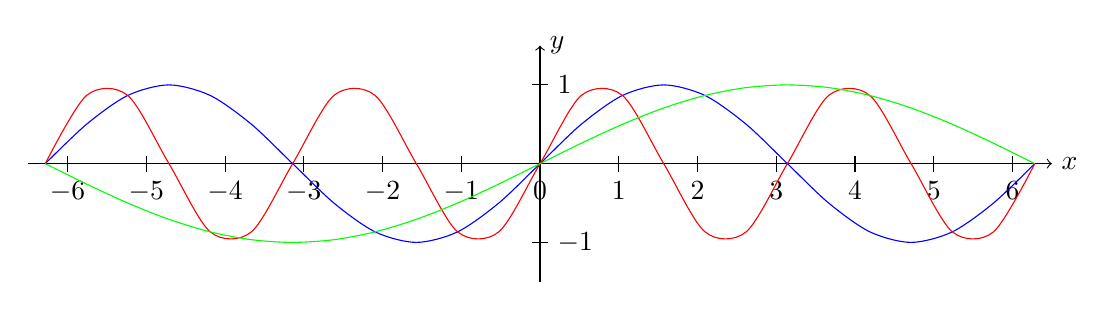
\begin{tikzpicture}[domain=-2*pi:2*pi,smooth]
    \draw [->] (-6.5,0) -- (6.5,0) node [right] {$ x $};
    \draw [->] (0,-1.5) -- (0,1.5) node [right] {$ y $};
    \foreach \x in {-6,...,6}{
      \draw (\x,-0.1) node [below] {$ \x $} -- (\x,0.1);
    }
    \foreach \y in {-1,1}{
      \draw (-0.1,\y) -- (0.1,\y) node [right] {$ \y $};
    }
    \draw [color=blue] plot (\x,{sin(deg(\x))});
    \draw [color=red] plot (\x,{sin(deg(2 * \x))});
    \draw [color=green] plot (\x,{sin(deg(0.5 * \x))});
  \end{tikzpicture}
	\caption{Skalierung der Sinus-Funktion (blau) mit dem Faktor $ 2 $ führt zu doppelt so schneller
  	Schwingung (roter Graph). Skalierung mit dem Faktor $ 0.5 $ bewirkt halb so schnelle
  	Schwingung (grüner Graph).}
	\label{fig:skalierung}
\end{figure}
\end{enumerate}
\end{definition}

\begin{remark}[Translations- und Skalierungsoperator] \leavevmode
\begin{enumerate}
\item der Translationsoperator verschiebt eine Funktion auf der $ x $-Achse um $ y $ Einheiten nach 
links oder rechts:
\par
\begin{center}
  \begin{tabular}{rl} \toprule
  Wert von $ y $ & Effekt auf $ f $ \\ \midrule
  $ y > 0 $ & Verschiebung nach \emph{links} \\
  $ y = 0 $ & Keine Verschiebung \\
  $ y < 0 $ & Verschiebung nach \emph{rechts} \\ \bottomrule
  \end{tabular}
\end{center}
\item Der Skalierungsoperator streckt oder staucht eine Funktion um den Faktor $ h $ und kann sie 
sogar an der $ y $-Achse spiegeln:\par
\begin{center}
  \begin{tabular}{rl} \toprule
  Wert von $ h $ & Effekt auf $ f $ \\ \midrule
  $ h > 1 $ & Stauchung \\
  $ h = 1 $ & Kein Effekt \\
  $ 0 < h < 1 $ & Streckung \\ \midrule
  $ h = 0 $ & Um Gottes Willen! Das ist pfui-gack. \\ \midrule
  $ -1 < h < 0 $ & Streckung und Spiegelung an der $ y $-Achse \\
  $ h = -1 $ & Nur Spiegelung an der $ y $-Achse \\
  $ h < -1 $ & Stauchung und Spiegelung an der $ y $-Achse \\ \bottomrule
  \end{tabular}
\end{center}
\item Die Definition des Skalierungsoperators ist recht ähnlich zur der des Abtastoperators mit
  Schrittweite $ h $. An dieser Stelle sollte betont werden, dass beide Operatoren nicht miteinander
  zu verwechseln sind! Der Abtastoperator liefert zu einem kontinuierlichen Signal $ f $
  ein diskretes Signal $ S_{h} \ f = (f(h \cdot \bullet))_{h \in \Z} $. Das $ h $ ist hier 
  variabel. Der Skalierungsoperator überführt ein kontinuierliches Signal $ f $ wieder in ein 
  kontinuierliches Signal $ \sigma_{h} \ f = f(h \cdot \bullet) $, welches eben um den Faktor $ h $ 
  gestreckt bzw.\ gestaucht wurde. $ h $ ist hier ein fester Wert.
\item Translation und Skalierung sind invertierbar, d.h.\ man kann ihre Auswirkungen wieder
rückgängig machen:
\[
  \tau_{y} \ (\tau_{-y} \ f) = \tau_{-y} \ (\tau_{y} \ f) = f \quad \text{und} \quad
  \sigma_{h} \ (\sigma_{1/h} \ f) = \sigma_{1/h} \ (\sigma_{h} \ f) = f.
\]
\end{enumerate}
\end{remark}

\begin{definition}[Faltung]
Seien $ f, g \in L(\R) $ und $ c,d \in l(\Z) $. Dann ist die Faltung zweier Funktionen definiert als
\[
  f * g \coloneqq \int_{\R} f(\bullet - t) \cdot g(t) \dif t \in L(\R)
\]
und die Faltung zweier Folgen als
\[
  c * d \coloneqq \sum_{k \in \Z} c(\bullet - k) \cdot d(k) \in l(\Z).
\]
Die Faltung einer Funktion $ f $ mit einer Folge $ c $ ist definiert durch
\[
  c * f \coloneqq f * c \coloneqq \sum_{k \in \Z} f(\bullet - k) \cdot d(k) \in L(\R).
\]
\end{definition}

\begin{remark}[Eigenschaften der Faltung]
Aus der Linearität des Integrals und den Gruppenoperationen auf $ \R $ lassen sich folgende 
Eigenschaften der Faltung für Funktionen oder Folgen $ f, g, h $ herleiten:
\begin{itemize}
\item Kommutativität: $ f * g = g * f $
\item Assoziativität: $ (f * g) * h = f * (g * h) $
\item Distributivität: $ f * (g + h) = f * g + f * h $
\item Skalare Multiplikation: $ a \cdot (f * g) = (a \cdot f) * g = f * (a \cdot g) $, wobei
  $ a \in \R $ eine beliebige Konstante ist.
\end{itemize}
\end{remark}
\begin{remark}[Interpretation der Faltung]
Die Faltung kann aufgefasst werden als Produkt zweier Funktionen oder Folgen, welches wieder eine
Funktion bzw. Folge liefert. Wie kann man sich die Faltung geometrisch vorstellen? Betrachten wir 
als Beispiel zwei Funktionen $ f $ und $ g $ und die Faltung $ f * g $. Was dabei passiert, ist 
Folgendes: Zunächst wird $ f $ durch $ f(\bullet - t) $ \emph{vertikal} gespiegelt. Wir halten 
anschließend die Funktion $ g $ fest und lassen $ f $ einmal komplett von ganz links nach 
ganz rechts über die $ x $-Achse wandern. Dort, wo sich $ f $ und $ g $ überlagern und eine große 
\enquote{Gemeinsamkeit} miteinander haben, wird auch das Integral groß. Dort, wo beide Funktionen 
keine große Gemeinsamkeit miteinander haben, wird das Integral klein. Die Faltung ist also eine 
Methode, um feststellen zu können, wie \emph{lokal} ähnlich (nicht global!) sich zwei Funktionen 
sind.

Je nachdem, welche Funktion man für $ g $ wählt, lassen sich mit der Faltung unterschiedliche 
interessante andere Funktionen erzeugen. Wikipedia meint, dass eine Faltung $ f * g $ einen
\enquote{gewichteten Mittelwert} von $ f $ darstellt, wobei die Gewichtung durch $ g $ vorgegeben 
ist. Diese Argumentation versteht man eigentlich erst, wenn man sich \emph{zyklische Faltungen}
anschaut, wo nicht über ganz $ \R $ integriert wird, sondern über ein Kompaktum. Dann wird das
Integral nämlich noch durch die Länge des Kompaktums dividiert, sodass man tatsächlich eine Art
Durschnitt hat. Und hey, das kommt uns doch jetzt irgendwie von der Definition der $ L_{2}(\R) $-
Funktionen bekannt vor!
\end{remark}

\begin{example}[Faltung]
Falten wir doch einmal die Rechtecksfunktion $ \chi_{[-1,1]} $ mit sich selbst. Man definiert
\[
  \chi_{[-1,1]}(x) = \begin{cases} 1, & x \in [-1,1] \\ 0, & \text{sonst}. \end{cases}
\]
Dann ist
\begin{align*}
   (\chi_{[-1,1]} * \chi_{[-1,1]})(x) 
&= \int_{\R} \chi_{[-1,1]}(x - t) \cdot \chi_{[-1,1]}(t) \dif t
 = \int_{\R} \chi_{[x - 1, x + 1]}(t) \cdot \chi_{[-1,1]}(t) \dif t \\
&= \int_{\R} \chi_{[x - 1, x + 1] \cap [-1,1]}(t) \dif t
 = \int_{[x - 1, x + 1] \cap [-1,1]} 1 \dif t \\
&= \begin{cases}
      \int_{-1}^{x+1} 1 \dif t = 2 + x, & -2 \leq x \leq 0, \\
      \int_{x-1}^{1} 1 \dif t = 2 - x, & 0 < x \leq 2, \\
      0, & \text{sonst},
   \end{cases} \\
&\eqcolon \Delta_{[-2,2]}(x).
\end{align*}
Man erhält also die Dreiecksfunktion auf dem Intervall $ [-2,2] $. Was bedeutet das? Naja, die
$ \Delta_{[-2,2]}(x) $ an der Stelle $ x $ gibt genau die Fläche an, die zwischen den beiden 
Rechtecksfunktionen gerade eingeschlossen wird, wenn man eine Rechtecksfunktion um $ x $ Einheiten
verschiebt. Im Fall von $ x = 0 $ überlappen sich beide Rechtecksfunktionen ganz genau, und deren
Flächeninhalt ist $ 2 $. Dies ist genau der Wert von $ \Delta_{[-2,2]}(2) $! Verschiebt man eine
Rechtecksfunktion um $ 1 $ Einheit nach links oder rechts, dann wird nur noch die Hälfte der
Fläche zwischen beiden Rechtecksfunktionen eingeschlossen, also Flächeninhalt $ 1 $. Und genau das
kommt bei $ \Delta_{[-2,2]}(x) $ heraus, wenn man $ x = 1 $ oder $ x = -1 $ einsetzt.

Die geometrische Interpretation einer Faltung ist also sehr vielfältig und hängt sehr stark von den
beiden Funktionen ab, die miteinander gefaltet werden, siehe Abbildung~\ref{fig:faltung}.
\begin{figure}[ht]
	\centering
	\includegraphics[width=0.7\linewidth]{Bilder/Faltung}
	\caption{Faltung der Rechtecksfunktion (orange und rot) mit sich selbst ergibt die 
  	Dreiecksfunktion (blau).}
	\label{fig:faltung}
\end{figure}
\end{example}

Nun kommen wir zu einem sehr wichtigen Teil der Vorlesung, nämlich zu den Eigenschaften der
Fourier-Transformation. Insbesondere wollen wir uns mit deren graphischer Deutung beschäftigen.
Faltungen werden in diesem Kontext auch eine sehr wichtige Rolle spielen, wenn wir die
Fourier-Transformierte besonders schnell berechnen wollen.

\begin{remark}[Eigenschaften der Fourier-Transformation und deren graphische Deutung]
  \label{prop:properties_fourier} \leavevmode
	 %%Hier könnten wir zu jeder Eigenschaft kurz schreiben was sie bedeuten und falls nötig oder 
	 %%möglich durch Bilder
	%%veranschaulichen
	\begin{description}
  	\item [Linearität] Die Fourier-Transformierte ist linear. Dies folgt sofort aus der Linearität 
  	des Integrals. Seien also $ f, g \in L_{1}(\R) $ und $ a, b \in \R $. Dann gilt:
    	\[
      	(a \cdot f + b \cdot g)^{\wedge} = a \cdot \widehat{f} + b \cdot \widehat{g}.
    	\]
    
    Bildliche Vorstellung: Multiplizieren wir eine Funktion $ f $ mit einer Konstanten $ a $, so
    ändert sich lediglich die Amplitude von $ f $. Die Frequenzen in der Funktion bleiben gleich,
    es kommen keine neuen Frequenzen hinzu und es fallen keine weg. Der \enquote{Anteil} der bereits
    vorhandenen Frequenzen wird nur anders gewichtet, nämlich mit dem Faktor $ a $ versehen. 
    Deshalb gilt $ (a \cdot f)^{\wedge} = a \cdot \widehat{f} $ (siehe hierfür auch 
    Abbildung~\ref{fig:FT_Linear}, linker Teil).
    
    Was hat es aber mit der Addition zweier Funktionen auf sich? Nun, wenn wir zwei Funktionen 
    addieren, so sollten sich auch die Anteile der Frequenzen addieren. Dies spiegelt sich genau in 
    der Identität $ (f + g)^{\wedge} = \widehat{f} + \widehat{g} $ wider 
    (Abbildung~\ref{fig:FT_Linear}, rechter Teil).
    
    Was passiert, wenn wir $ f = g $ setzen? Dann sollte der Anteil jeder Frequenz doppelt so groß
    sein wie vorher. Und in der Tat: Wir können jetzt entweder sagen 
    $ (f + f)^{\wedge} = \widehat{f} + \widehat{f} = 2 \widehat{f} $ oder
    $ (f + f)^{\wedge} = (2f)^{\wedge} = 2 \widehat{f} $. In beiden Fällen kommt das gleiche raus.
    \begin{figure}[ht]
      \centering
      \begin{minipage}{0.49\linewidth}
        \centering
        \includegraphics[width=\linewidth]{Bilder/FT_Linear1}
      \end{minipage}
      \begin{minipage}{0.49\linewidth}
        \centering
        \includegraphics[width=\linewidth]{Bilder/FT_Linear2}
      \end{minipage}
      \caption{Links: Änderung der Amplitude der Sinus-Funktion bei gleichbleibender Frequenz.
        Rechts: Bei Addition der Sinus- und Cosinus-Funktion addieren sich auch die Frequenzen.}
      \label{fig:FT_Linear}
    \end{figure}
    
		\item [Translation (Zeitverschiebung)] Für $ f \in L_1(\R) $ und $ y \in \R $ gilt:
		\[ 
    		(\tau_{y} \ f)^{\wedge}(\xi) 
  		= \left( f(\bullet + y) \right)^{\wedge}(\xi) 
  		= e^{iy\xi}\widehat{f}(\xi), \quad \xi \in \R.
    \]
		Wie bereits oben erwähnt verschiebt eine Translation eine Funktion um den Wert $ y $. 
		Verschiebt man nun die ursprüngliche Funktion des Signal, sollte sich an den Anteilen der 
		Frequenzen $ \xi $ nichts ändern. Wo kommt aber nun dieser seltsame Faktor $ e^{iy\xi} $ her? 
		Dazu müssen wir uns wieder in Erinnerung rufen, dass sich die Fourier-Transformation auch so 
		schreiben lässt: $ \int_{\R} f(t) \cos(\xi t) \dif t - i \int_{\R} f(t) \sin(\xi t) \dif t $.\\
		$ \rightarrow $ Es gibt einen Imaginärteil und einen Realteil. Durch die Translation ändert 
		sich nur die Aufteilung zwischen diesen zwei Teilen. Der Gesamtanteil bleibt gleich. Diese 
		Umverteilung geschieht durch den Vorfaktor $ e^{iy\xi} $. (Dies bezeichnet man auch als
		\emph{Frequenz-Modulation}). 
		
  \begin{figure}[ht]
      \centering
      \begin{minipage}{0.49\linewidth}
        \centering
        \includegraphics[width=\linewidth]{Bilder/Rechteck1}
      \end{minipage}
      \begin{minipage}{0.49\linewidth}
        \centering
        \includegraphics[width=\linewidth]{Bilder/Rechteck2}
      \end{minipage}
      \caption{Links: Rechtecksfunktion und deren Fourier-Transformierte. Rechts: Die um $ 1 $
        nach links verschobene Rechtecksfunktion und deren Fourier-Transformierte mit Real- und 
        Imaginärteil separat geplottet (Realteil rot, Imaginärteil grün). Gut sichtbar ist die 
        Phasenverschiebung zwischen Sinus und Cosinus.}
      \label{fig:Rechteck12}
    \end{figure}
    \begin{figure}[ht]
      \centering
      \begin{minipage}{0.49\linewidth}
        \centering
        \includegraphics[width=\linewidth]{Bilder/Rechteck3}
      \end{minipage}
      \begin{minipage}{0.49\linewidth}
        \centering
        \includegraphics[width=\linewidth]{Bilder/Rechteck4}
      \end{minipage}
      \caption{Links: Fourier-Transformierte der Rechtecksfunktion (blau) und der verschobenen
        Rechtecksfunktion (Realteil rot, Imaginärteil grün). Rechts: Fourier-Transformation der
        Rechtecksfunktion (blau) und der verschobenen Rechtecksfunktion im Absolutbetrag (rot).}
      \label{fig:Rechteck34}
    \end{figure}
		
		Betrachten wir $ \widehat{f} $ als Vektor in der komplexen Zahlenebene, so führt der Faktor $ 
		e^{iy\xi} $ lediglich dazu, dass die 
		der Vektor um den Winkel $ y \cdot \xi $ im Uhrzeigersinn gedreht wird. D.h.\ an den Anteilen
		der Frequenzen ändert sich im Absolutbetrag nichts. Schließlich ist ja auch $ |e^{iy\xi}| = 1 $.
		
		Als veranschaulichendes Beispiel diene hier die Rechtecks-Funktion $ \chi_{[-1,1]} $ mit
		ihrer Fourier-Transformierten $ 2\sin(x) / x $. Wird die Rechtecks-Funktion um eine Einheit 
		nach 
		links verschoben, so wird die Fourier-Transformierte mit dem Vorfaktor $ e^{i\xi} $ versehen,
		also
		\[   (\tau_{1}\chi_{[-1,1]})^{\wedge}(\xi)
  		 = \left( \chi_{[-1,1]}(\bullet + 1) \right)^{\wedge}(\xi)
  		 = \widehat{\chi}_{[-2,0]}(\xi)
  		 = e^{i\xi} \cdot \frac{2 \sin(\xi)}{\xi}.
  	\]
  	Abbildung~\ref{fig:Rechteck12} zeigt die Rechtecksfunktion und die verschobene 
  	Rechtecksfunktion, sowie deren Fourier-Transformierte. Wir stellen zunächst fest, dass die
  	Rechtecksfunktion eine vollständig reelle Fourier-Transformierte besitzt und die verschobene
  	Rechtecksfunktion eine reell- und komplexwertige Fourier-Transformierte. Dies zeigt ganz 
  	deutlich, dass sich die Aufteilung der Frequenzen zwischen Sinus und Cosinus verschoben hat. Die
  	interessante Frage ist aber nun: Hat sich an den Anteilen der Frequenzen im Ganzen etwas 
  	geändert? Die Antwort liefert Abbildung~\ref{fig:Rechteck34}. Im Absolutbetrag sind nämlich 
  	beide Fourier-Transformationen identisch. D.h.\ die Frequenzanteile sind im Ganzen gleich
  	geblieben. Dies hätte man auch schon so sehen können:
  	\[
    	  \left| (\tau_{1}\chi_{[-1,1]})^{\wedge}(\xi) \right|
    	= \left| e^{i\xi} \cdot \widehat{\chi}_{[-1,1]}(\xi) \right|
    	= \left| e^{i\xi} \right| \cdot \left| \widehat{\chi}_{[-1,1]}(\xi) \right|
    	= 1 \cdot \left| \widehat{\chi}_{[-1,1]}(\xi) \right|
    	= \left| \widehat{\chi}_{[-1,1]}(\xi) \right|.
  	\]
  	
  	Also ganz kurz und knapp: Verschiebung im Zeit-/Ortsbereich führt zu Modulation im
  	Frequenzbereich.
  	
  	Übrigens: Der Realteil der Fourier-Transformierten ist immer achsensymmetrisch zur $ y $-Achse,
  	weil der Cosinus achsensymmetrisch zur $ y $-Achse ist, und der Imaginärteil ist 
  	punktsymmetrisch um den Ursprung, weil der Sinus punktsymmetrisch um den Ursprung ist.
 
		\item [(Zeit-)Skalierung] Sei $ f \in L_{1}(\R) $ und $ h \neq 0 $. Dann gilt
  		\[
      		(\sigma_{h} \ f)^{\wedge}(\xi) 
      	= f(h \cdot \bullet)^{\wedge}(\xi) 
      	= \frac{1}{|h|} \widehat{f} \left( \frac{\xi}{h} \right), \quad \xi \in \R.
  		\]
  	Durch den Skalierungsoperator wird eine Funktion im Zeit-/Ortsbereich in Richtung der $x$-Achse 
  	gestaucht oder gestreckt (anders ausgedrückt: Die Periodenlänge ändert sich). Damit ändern sich
  	auch die im Signal enthaltenen Frequenzen. Beispiel anhand des Sinus: Wird die Periodenlänge 
    halbiert, so verdoppelt sich doch die Frequenz, denn der Sinus schwingt jetzt doppelt so 
    schnell. In diesem Kontext ist die Frequenz der Reziprokwert der Periodenlänge.
    
    \begin{figure}[ht]
          \centering
          \begin{minipage}{0.49\linewidth}
            \centering
            \includegraphics[width=\linewidth]{Bilder/FT_Skalierung_Zeit}
          \end{minipage}
          \begin{minipage}{0.49\linewidth}
            \centering
            \includegraphics[width=\linewidth]{Bilder/FT_Skalierung_Freq}
          \end{minipage}
          \caption{Links: Rechtecksfunktion (blau) und gestauchte Rechtecksfunktion (rot). 
          Rechts:
            Fourier-Transformationen zu den Rechtecksfunktionen (in gleicher Farbe).}
          \label{fig:FT_Skalierung}
        \end{figure}
    
    Können wir diese Analogie auch auf die Fourier-Transformation übertragen? Betrachten wir ein
    weiteres Mal die Rechtecksfunktion. Skalieren wir diese mit einem Faktor von $ h = 2 $ und 
    bilden davon die Fourier-Transformation, so erhalten wir:
    \[
        (\sigma_{2} \ \chi_{[-1,1]})^{\wedge}(\xi)
      = \frac{1}{2} \widehat{\chi}_{[-1,1]} \left( \frac{\xi}{2} \right) 
      = \frac{2}{\xi} \sin \left( \frac{\xi}{2} \right).
    \]
    Abbildung~\ref{fig:FT_Skalierung} zeigt die eben angesprochenen Funktionen. Das 
    $ \xi /2 $ im Argument von $ (\sigma_{2} \ \chi_{[-1,1]})^{\wedge} $ führt dazu, dass die
    Fourier-Transformation auseinander gezogen wird. Durch den Vorfaktor $ 2 / \xi $ verringert sich
    zudem die Amplitude. Dies macht auch Sinn, denn durch das Zusammenstauchen einer Funktion im
    Ortsbereich schwingt sie ja schneller, sie wird hochfrequenter. Das entspricht genau dem
    Auseinanderziehen der Fourier-Transformation. Es wird mehr Anteil in den hochfrequenten Bereich
    verlagert. Gleichzeitig wird der Anteil der niedrigen Frequenzen (die sich im Frequenzbereich 
    um den Ursprung konzentrieren) geringer, was dem Plattdrücken der Fourier-Transformierten 
    entspricht.
    
    Man stellt fest: Für große Werte von $ h $ konzentriert sich die Funktion im Zeitbereich stark 
    um den Ursprung, sie wird gestaucht und hochfrequenter. Im Frequenzbereich führt dies dazu,
    dass die Fourier-Transformation gestreckt (auseinander gezogen) und platt gedrückt wird.
    Umgekehrt führen kleine Werte von $ h $ dazu, dass die Funktion im Ortsbereich gestreckt wird,
    also niederfrequenter wird. Die Fourier-Transformation wird um den Ursprung zusammengedrückt und
    schlägt stärker aus.
    
		\item [Faltung] Für $ f, g \in L_{1}(\R) $ bzw.\ $ c, d \in l_{1}(\Z) $ sind 
  	$ f * g \in L_{1}(\R) $, $ c * d \in l_{1}(\Z) $ und $ f * c \in L_{1}(\R) $ und es gilt:
    \[
      (f * g)^{\wedge}(\xi) = \widehat{f}(\xi) \widehat{g}(\xi), \quad
      (c * d)^{\wedge}(\xi) = \widehat{c}(\xi) \widehat{d}(\xi)  \quad \text{und} \quad
      (f * c)^{\wedge}(\xi) = \widehat{f}(\xi) \widehat{c}(\xi).
    \]
    Eine Faltung im Zeitbereich gibt ja so etwas wie die Übereinstimmung zwischen den beiden 
    Funktionen an, und die Multiplikation im Frequenzbereich kann man sich nun vorstellen als
    Übereinstimmung der Frequenzen der beiden Funktionen.
    
    \emph{Eine Faltung im Zeitbereich wird also überführt in eine Multiplikation im   
    Frequenzbereich.} Dies ist eine extrem wichtige Eigenschaft der Fourier-Transformation. Dies hat
    im Wesentlichen zwei Gründe:
    \begin{enumerate}
    \item Die Berechnung einer Faltung zweier Funktionen ist normalerweise viel aufwendiger als die 
        beiden Funktionen einfach punktweise zu multiplizieren (es sind hier weniger Operationen
        auszuführen).
    \item Außerdem weist das Produkt eine höhere numerische Stabilität auf als die Faltung.
    \end{enumerate}
    Diese Eigenschaften kann man sich zunutze machen, um Filter effizient zu implementieren, und
    dabei ist von der Schnellen Fourier-Transformation (FFT) noch gar nicht die Rede.
    
    Weil es so schön ist, hier der Faltungsbeweis für den Fall, dass zwei Funktionen
    $ f,g \in L_{1}(\R) $ gegeben sind:
    \begin{align}
       (f * g)^{\wedge}(\xi)
    &= \int_{\R} (f * g)(x) e^{-i\xi x} \dif x \tag{Def.\ Fourier-Transf.} \\
    &= \int_{\R} \left( \int_{\R} f(t) g(x - t) \dif t \right) e^{-i\xi x} \dif x 
        \tag{Def.\ Faltung} \\
    &= \int_{\R} \int_{\R} f(t) g(x - t)  e^{-i\xi x} \dif x \dif t
        \tag{Tonelli} \\
     &= \int_{\R} \int_{\R} f(t) g(s)  e^{-i\xi (t + s)} \dif s \dif t
            \tag{Subst. $ s \coloneqq x - t $, $ \dif s = \dif x $} \\
    &= \left( \int_{\R} f(t) e^{-i\xi t} \dif t \right)
       \left( \int_{\R} g(s) e^{-i\xi s} \dif s \right) \tag{Arithmetik \& Tonelli} \\
    &= \widehat{f}(\xi) \cdot \widehat{g}(\xi). \tag{Def.\ Fourier-Transf.}
    \end{align}

		\item [Ableitungseigenschaften] Sind $ f, f' \in L_{1}(\R) $, dann gilt
    \[
      \left( \dod{f}{x} \right)^{\wedge}(\xi) = i\xi \widehat{f}(\xi), \quad \xi \in \R.
    \]
    Sind $ f, xf \in L_{1}(\R) $, dann ist $ \widehat{f} $ differenzierbar und es gilt
    \[
      \dod{\widehat{f}(\xi)}{\xi} = (-ix f)^{\wedge}(\xi).
    \]
    Diese Eigenschaften sind vor allem nützlich fürs Rechnen.
    
		\item [Inverse Fourier-Transformation] Sind $ f, \widehat{f} \in L_{1}(\R) $, dann ist
		\[
  		f(x) = (\widehat{f})^{\vee}(x) \coloneqq 
    		\frac{1}{2\pi} \int_{\R} \widehat{f}(\vartheta) \ e^{i x \vartheta} \dif \vartheta,
    		\qquad x \in \R.
		\]
		Die Operation $ f \mapsto f^{\vee} \coloneqq \frac{1}{2\pi} f^{\wedge}(-\bullet) $ bezeichnet
		man als inverse Fourier-Transformation.
		
		Sind $ c \in l_{1}(\R) $ und $ \widehat{c} \in L_{1}(\T) $, dann ist
		\[
		  c(k) = (\widehat{c})^{\vee}(k) \coloneqq
  		  \frac{1}{2\pi} \int_{\T} \widehat{c}(\xi) e^{ik\xi} \dif \xi,
  		  \qquad k \in \Z.
		\]
		Die Operation $ c \mapsto c^{\vee} $ bezeichnet man als inverse Fourier-Transformation.
		
		Dass die Nützlichkeit einer Transformation stark
		davon abhängt, ob bzw.\ unter welchen Voraussetzungen diese wieder rückgängig gemacht werden 
		kann, braucht an dieser Stelle nicht weiter betont zu werden. In unserem Fall müssen beide
		Funktionen $ f, \widehat{f} \in L_{1}(\R) $ sein. Setzen wir beispielsweise
		$ f = \chi_{[-1,1]} $, so erhalten wir i.W.\ die $ \sinc $-Funktion als Fourier-Transformierte.
		Diese ist aber keine $ L_{1}(\R) $-Funktion mehr und deshalb ist die Fourier-Transformation hier
		insbesondere nicht invertierbar! Aber das kommt Gott sei Dank nicht so häufig vor.
		
		Ist $ c \in l_{1}(\Z) $, dann gilt auch $ \widehat{c} \in L_{1}(\T) $, denn
		\begin{align*}
  		 \norm{\widehat{c}}_{\T, 1}
		&= \int_{\T} |\widehat{c}(t)| \dif t
		 = \int_{\T} \left| \sum_{k \in \Z} c(k) e^{-ikt} \right| \dif t \\
		&\leq \int_{\T} \sum_{k \in \Z} |c(k)| \underbrace{|e^{-ikt}|}_{= 1} \dif t
		 = \int_{\T} \underbrace{\sum_{k \in \Z} |c(k)|}_{= \norm{c}_{1}} \dif t \\
		&= \int_{\T} \norm{c}_{1} \dif t
		 = \underbrace{\norm{c}_{1}}_{< \infty} \underbrace{\int_{\T} 1 \dif t}_{< \infty} \\
		&< \infty.
		\end{align*}
		Mit anderen Worten, die Fourier-Transformation für Folgen ist im Gegensatz zu der für Funktionen
		\emph{immer} invertierbar.
		
		Dass die Formel für die Inverse Fourier-Transformation den Vorfaktor $ 1 / 2\pi $ beinhaltet,
		liegt daran, dass wir die Formel für die Fourier-Transformation in 
		Definition~\ref{def:Fourier-Transformation} mit keinen Vorfaktor versehen haben. Dies ist aber 
		nur Normierung. Wir hätten auch in Definition~\ref{def:Fourier-Transformation} mit
		$ 1 / \sqrt{2\pi} $ normieren können, dann wäre dieser Faktor jetzt auch bei der Inversen
		Fourier-Transformation aufgetaucht und wir hätten eine schöne Isometrie.
	\end{description}
\end{remark}

\begin{example}[Inverse Fourier-Transformation]
Wir berechnen die Fourier-Transformation der Gauß-Funktion
\[
  f(x) = \exp(-x^{2}), \quad x \in \R.
\]
Der Nachweis $ f \in L_{1}(\R) $ sei dabei dem Leser zur Übung überlassen. Es sei aber soviel 
gesagt, dass
\[
  \int_{\R} f(x) \dif x = \sqrt{\pi}.
\]
Es gilt
\begin{align*}
   \widehat{f}(\xi)
&= \int_{\R} f(x) \exp(-i\xi x) \dif x
 = \int_{\R} \exp(-x^{2}) \exp(-i\xi x) \dif x
 = \int_{\R} \exp(-(x^{2} + i\xi x)) \dif x \\
&= \int_{\R} \exp(-(x^{2} + i\xi x - \xi^{2} / 4) - \xi^{2}/4 ) \dif x
 = \int_{\R} \exp(-(x + i\xi / 2)^{2}) \exp(-\xi^{2}/4) \dif x.
\end{align*}
Die Substitution $ u \coloneqq x + i\xi / 2 $, $ \dif u = \dif x $ liefert weiter
\[
    \exp(-\xi^{2}/4) \underbrace{ \int_{\R} \exp(-u^{2}) \dif u }_{=\sqrt{\pi}}
  = \sqrt{\pi} \exp(-\xi^{2}/4).
\]
Wir haben also gezeigt, dass $ \widehat{f}(\xi) = \sqrt{\pi} \exp(-\xi^{2}/4) $. Die
Fourier-Transformierte der Gauß-Funktion ist also i.W.\ bis auf Normierung die Gauß-Funktion selbst.
Man kann sich leicht überlegen, dass auch $ \widehat{f}(\xi) \in L_{1}(\R) $. Damit können wir
die Inverse Fourier-Transformation berechnen. Dabei sollte wieder die ursprüngliche Funktion $ f $
herauskommen. Also:
\begin{align*}
   \left( \widehat{f} \right)^{\vee}(x)
&= \frac{1}{2\pi} \int_{\R} \widehat{f}(\xi) \exp(i\xi x) \dif \xi
 = \frac{1}{2\pi} \int_{\R} \sqrt{\pi} \exp(-\xi^{2}/4) \exp(i\xi x) \dif \xi \\
&= \frac{1}{2\sqrt{\pi}} \int_{\R} \exp(-\xi^{2}/4 + i\xi x) \dif \xi
 = \frac{1}{2\sqrt{\pi}} \int_{\R} \exp(- (\xi^{2}/4 - i\xi x - x^{2}) - x^{2}) \dif \xi \\
&= \frac{1}{2\sqrt{\pi}} \int_{\R} \exp(-(\xi/2 - ix)^{2}) \exp(-x^{2}) \dif \xi \\
&= \frac{1}{2\sqrt{\pi}} \exp(-x^{2}) \int_{\R} \exp(-(\xi/2 - ix)^{2}) \dif \xi.
\end{align*}
Die Variablensubstitution $ u \coloneqq \xi / 2 - ix $, $ \dif \xi = 2 \dif u $ liefert 
daraus schließlich
\[
    \frac{1}{2\sqrt{\pi}} \exp(-x^{2}) \underbrace{ \int_{\R} 2\exp(-u^{2}) \dif u }_{=\sqrt{\pi}}
  = \frac{1}{\sqrt{\pi}} \sqrt{\pi} \exp(-x^{2})
  = \exp(-x^{2}) = f(x),
\]
wie behauptet.
\end{example}

\begin{remark}[Zusammenhang zwischen Symmetrie einer Funktion und deren Fourier-Transformierter]
Ist $ f \in L_{1}(\R) $ eine symmetrische Funktion, d.h.\ $ f(x) = f(-x) $ für alle $ x \in \R $, 
dann ist auch $ \widehat{f} $ symmetrisch und reell. Denn es gilt:
\[
   \widehat{f}(\xi)
 = \int_{\R} f(x) e^{-i\xi x} \dif x
 = \int_{\R} f(x) \cos(\xi x) \dif x - i \int_{\R} f(x) \sin(\xi x) \dif x.
\]
Für das rechte Integral gilt
\begin{align}
   \int_{\R} f(x) \sin(\xi x) \dif x \notag
&= \int_{-\infty}^{0} f(x) \sin(\xi x) \dif x + \int_{0}^{\infty} f(x) \sin(\xi x) \dif x 
     \notag \\
&= - \int_{\infty}^{0} f(-t) \sin(-\xi t) \dif t + \int_{0}^{\infty} f(x) \sin(\xi x) \dif x
     \tag{Subst.\ $ t \coloneqq -x $, $ \dif t = -\dif x $} \\
&= \int_{0}^{\infty} f(t) \sin(-\xi t) \dif t + \int_{0}^{\infty} f(x) \sin(\xi x) \dif x
     \tag{$ f(x) = f(-x) $} \\
&= - \int_{0}^{\infty} f(x) \sin(\xi x) \dif x + \int_{0}^{\infty} f(x) \sin(\xi x) \dif x
     \tag{$ \sin(-x) = -\sin(x) $} \\
&= 0 \notag,
\end{align}
und damit
\[
   \widehat{f}(\xi)
 = \int_{\R} f(x) \cos(\xi x) \dif x \in \R, \qquad
   \widehat{f}(- \xi) = \widehat{f}(\xi),
\]
wie behauptet.

Auf gleiche Weise lässt sich zeigen, dass die Fourier-Transformation zu einer antisymmetrischen 
Funktion rein imaginär ist.
\end{remark}

\begin{proposition}[Riemann-Lebesgue-Lemma]\label{prop:Riemann-Lebesgue}
Ist $ f \in L_{1}(\R) $, so ist
\[
  \lim\limits_{\xi \to \infty} \widehat{f}(\xi) = 0.
\]
\end{proposition}

\begin{remark}[Riemann-Lebesgue-Lemma]
Die Kernessenz von Lemma~\ref{prop:Riemann-Lebesgue} ist, dass die Fourier-Transformation 
$ \widehat{f} $ einer Funktion $ f $ im Unendlichen verschwindet. Der Anteil der sehr großen
Frequenzen nimmt immer weiter ab, je größer die Frequenzen werden. Aber Achtung: Der Satz macht
keine Aussage darüber, wie schnell das Abklingverhalten von $ \widehat{f} $ ist! Daher gilt im
allgemeinen \emph{nicht}, dass $ \widehat{f} \in L_{1}(\R) $, wenn $ f \in L_{1}(\R) $. Das haben
wir ja bereits gesehen anhand der charakteristischen Funktion.
\end{remark}

\begin{definition}[Fourier-Koeffizienten und Fourier-Reihe]
Zu $ f \in L_{1}(\T) $ sind die \emph{Fourier-Koeffizienten} definiert als
\[
  f_{k} \coloneqq \frac{1}{2\pi} \int_{\T} f(t) e^{-ikt} \dif t, \qquad k \in \Z,
\]
und die \emph{Fourier-Reihe} zu $ f $ als
\[
    \mathcal{F}f \coloneqq \sum_{k \in \Z} f_{k} e^{ik\bullet}
\]
\end{definition}

\begin{remark}[Fourier-Koeffizienten und Fourier-Reihe]\leavevmode
\begin{itemize}
\item Die Fourier-Reihe $ \mathcal{F}f $ ist $ 2\pi $-periodisch und unter bestimmten
  Voraussetzungen die Fourier-Transformation der Folge der Fourier-Koeffizienten: 
  $ \mathcal{F}f = \widehat{f_{k}} $.
\item Es ist aber im allgemeinen nicht garantiert, dass die Fourier-Reihe von $ f $ konvergiert, 
  oder dass sie im Falle der Konvergenz gegen $ \widehat{f} $ konvergiert.
\end{itemize}
\end{remark}

\begin{proposition}[Poisson'sche Summenformel]
Für $ f \in L_{1}(\R) $ ist
\[
  \sum_{k \in \Z} f(2k\pi) = \frac{1}{2\pi} \sum_{k \in \Z} \widehat{f}(k)
  \qquad \text{und} \qquad
  \sum_{k \in \Z} f(k) = \sum_{k \in \Z} \widehat{f}(2k\pi).
\]
\end{proposition}

\begin{proposition}[Parseval/Plancherel]
Für $ f, g \in L_{1}(\R) \cap L_{2}(\R) $ ist
\[
    \int_{\R} f(t) \ g(t) \dif t 
  = \frac{1}{2\pi} \int_{\R} \widehat{f}(\vartheta) \ \overline{\widehat{g}(\vartheta)}
      \dif \vartheta.
\]
Insbesondere gilt mit $ f = g $
\[
  \norm{f}_{2} = \frac{1}{\sqrt{2\pi}} \norm{\widehat{f}}_{2}.
\]
\end{proposition}

\begin{remark}[Parseval/Plancherel]
Aus dem vorherigen Satz lassen sich gleich mehrere interessante Schlüsse ziehen:
\begin{itemize}
\item Die Fourier-Transformation ist bis auf Normierung eine Isometrie auf $ L_{2} $. Hätten wir in 
  Definition~\ref{def:Fourier-Transformation} die Normierung $ 1 / \sqrt{2\pi} $ verwendet, so
  könnten wir nun schreiben:
  \[
    \norm{f}_{2} = \norm{\widehat{f}}_{2}
  \]
  und wir hätten die perfekte Symmetrie. Dies ließe auch die Interpretation zu, dass die 
  Fourier-Transformation energieerhaltend ist (die Zwei-Norm wird ja auch als Energienorm 
  bezeichnet). Da lacht der Physiker \smiley.
\item Der Satz von Parseval/Plancherel liefert ein Skalarprodukt von Funktionen
  $ f, g \in L_{1}(\R) \cap L_{2}(\R) $:
  \[
      \langle f, g \rangle 
    = \int_{\R} f(t) \ g(t) \dif t
    = \frac{1}{2\pi} \int_{\R} \widehat{f}(\vartheta) \ \overline{\widehat{g}(\vartheta)}
          \dif \vartheta.
  \]
  Das bedeutet, wir dürfen uns insbesondere der schönen Rechenregeln für Skalarprodukte bedienen
  (Linearität, Symmetrie usw.).
\item Wie wir bereits gesehen haben, gibt es Funktionen in $ L_{1}(\R) $, für die die 
  Inversionsformel der Fourier-Transformation nicht gilt. Daher wäre es schön, die
  Fourier-Transformation auf andere Funktionenräume wie den $ L_{2}(\R) $ zu verallgemeinern. Dabei
  können wir ausnutzen, dass $ L_{1}(\R) \cap L_{2}(\R) $ dicht in $ L_{2}(\R) $ liegt. Wir
  definieren zu $ f \in L_{2}(\R) $ eine Folge
  \[
    f_{n} \coloneqq \chi_{[-n,n]} \cdot f \quad \in L_{1}(\R) \cap L_{2}(\R), \qquad n \in \N,
  \]
  welche für $ n \to \infty $ in der Norm $ \norm{\bullet}_{2} $ gegen $ f $ konvergiert.
  $ \widehat{f_{n}} $ ist dann eine Cauchy-Folge, die wegen der Dichtheit von $ L_{1}(\R) \cap 
  L_{2}(\R) $ in $ L_{2}(\R) $ gegen eine Funktion in $ L_{2}(\R) $ konvergiert. Diese Funktion 
  nennen wir $ \widehat{f} $:
  \[
      \widehat{f} \coloneqq \lim\limits_{n \to \infty} \widehat{f_{n}}
    = \lim\limits_{n \to \infty} \left( \chi_{[-n,n]} \cdot f \right)^{\wedge}
    = \lim\limits_{n \to \infty} \int_{-n}^{n} f(x) \exp(-i\xi x) \dif x,
      \qquad f \in L_{2}(\R).
  \]
  
\end{itemize}
\end{remark}

\TODO{Sollen wir mal ein Beispiel rechnen zu einer FT in $ L_{2} $?}